\section{Ripple Counters}
\label{sec:ripple-counter}

A register that goes through a prescribed sequence of states upon the application of input pulses is called a \textit{counter}. The input pulses may be clock pulses, or they may originate from some external source and may occur at a fixed interval of time or at random. The sequence of states may follow the binary number sequence or any other sequence of states. A counter that follows the binary number sequence is called a \textit{binary counter}.

Counters are available in two categories:
\begin{itemize}
  \item Ripple counters
  \item Synchronous counters
\end{itemize}

In a \textit{ripple counter}, a flip-flop output transition serves as a source for triggering other flip-flops. In other words, the clock input of some or all flip-flops are triggered, not by the common clock pulses, but rather by the transition that occurs in other flip-flop outputs.

In a \textit{synchronous counter}, the clock inputs of all flip-flops receive the common clock.

\subsection{Binary Ripple Counter}
\label{subsec:binary-ripple-counter}

A binary ripple counter consists of a series connection of complementing flip-flops, with the output of each flip-flop connected to the $C$ input of the next higher order flip-flop. 

\columnbreak

\noindent The flip-flop holding the least significant bit receives the incoming count pulses. The logic diagram of two 4-bit binary ripple counters is shown in Fig. 8.

\end{multicols}

\begin{figure}[H]
  \centering
  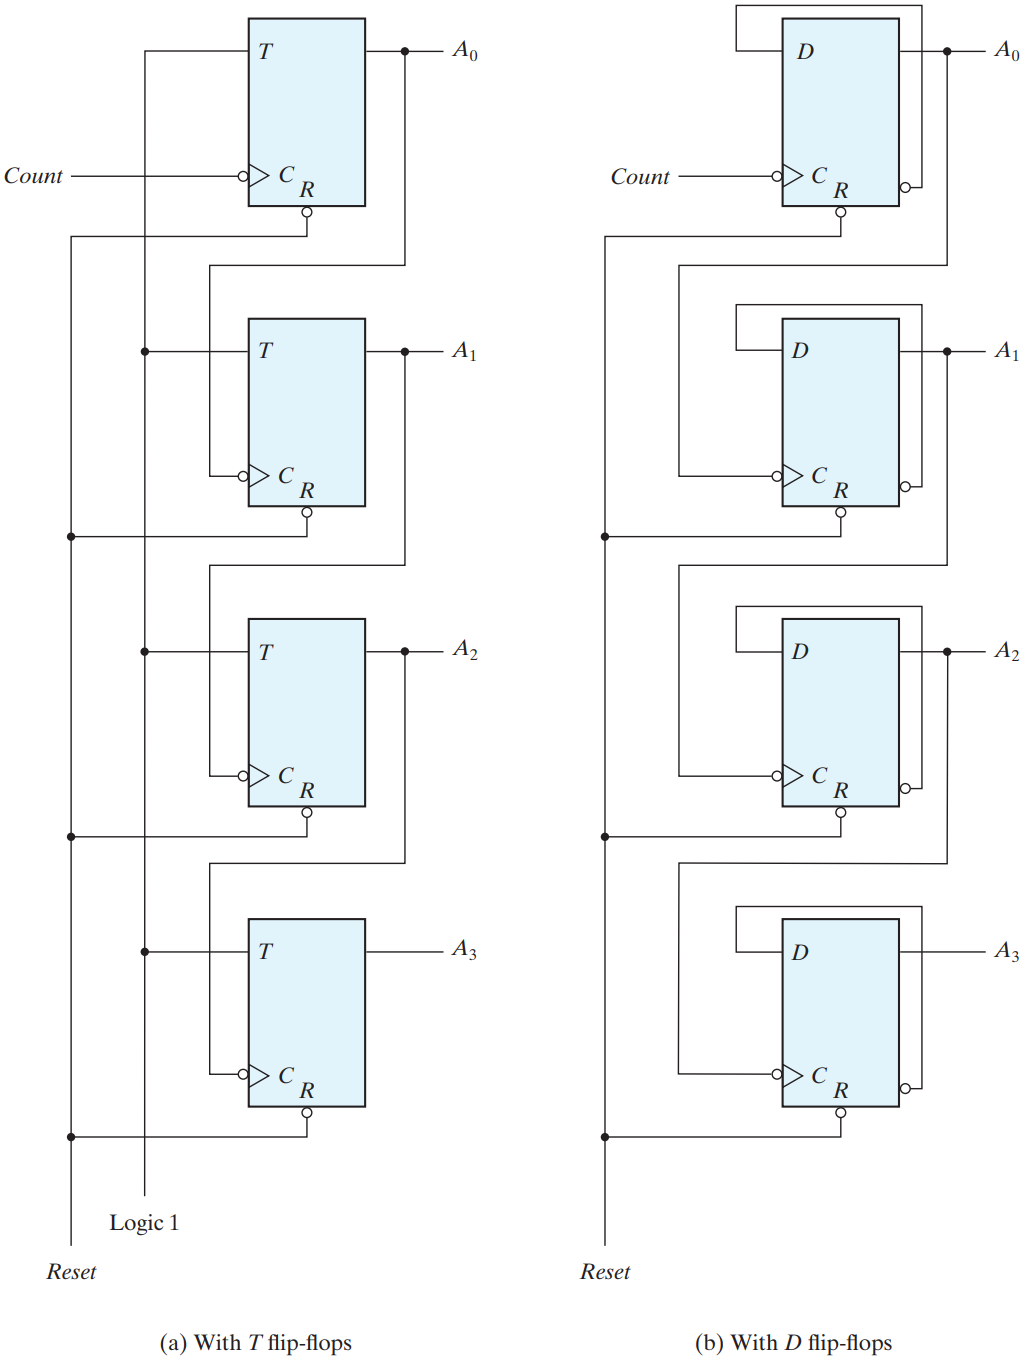
\includegraphics[width=.65\linewidth]{img/fig-6.8.png}
  \caption{Four-bit binary ripple counter}
  \label{fig:6.8}
\end{figure}

\begin{multicols}{2}
\setlength{\columnsep}{1.5cm}
\setlength{\columnseprule}{0.2pt}

To understand the operation of the four-bit binary ripple counter, refer to the first nine binary numbers listed in Table 6.4. The count starts with binary 0 and increments by 1 with each count pulse input. The count starts with binary 0 and increments by 1 with each count pulse input. After the count of 15, the counter goes back to 0 to repeat the count. The least significant bit, $A_0$, is complemented with each count pulse  input. Every time that $A_0$ goes from 1 to 0, it complements $A_1$. Every time that $A_1$ goes from 1 to 0, it complements $A_2$. Every time that $A_2$ goes from 1 to 0, it complements $A_3$ and so on for any other higher order bits of a ripple counter.

\begin{figure}[H]
  \centering
  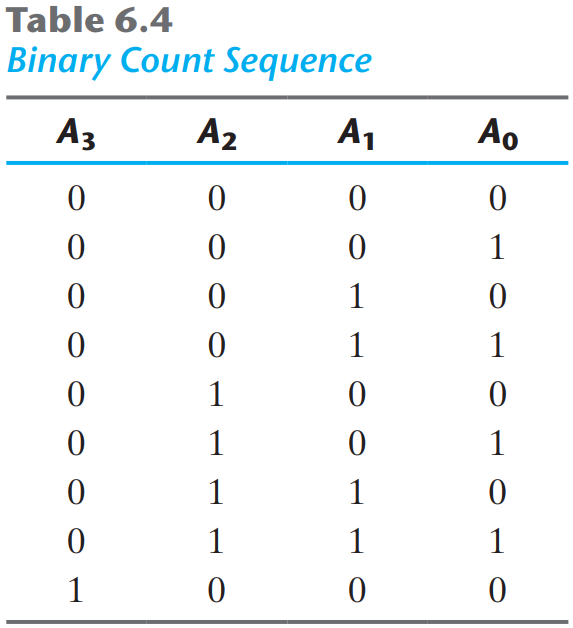
\includegraphics[width=.5\linewidth]{img/table-6.4.png}
  \label{table:6.4}
\end{figure}

A binary counter with a reverse count is called a \textit{binary countdown counter}. In a countdown counter, the binary count is decremented by 1 with every input count pulse. The count of a four-bit countdown counter starts from binary 15 and continues to binary counts 14, 13, 12, . . . , 0 and then back to 15.


\subsection{BCD Ripple Counter}
\label{subsec:bcd-ripple-counter}

A decimal counter follows a sequence of 10 states and returns to 0 after the count of 9. Such a counter must have at least four flip-flops to represent each decimal digit, since a decimal digit is represented by a binary code with at least four bits.

If the BCD code is used, the sequence of states is as shown in the state diagram of Fig. 9. A decimal counter is similar to a binary counter, except that the state after 1001 (the code for decimal digit 9) is 0000 (the code for decimal digit 0).

\begin{figure}[H]
  \centering
  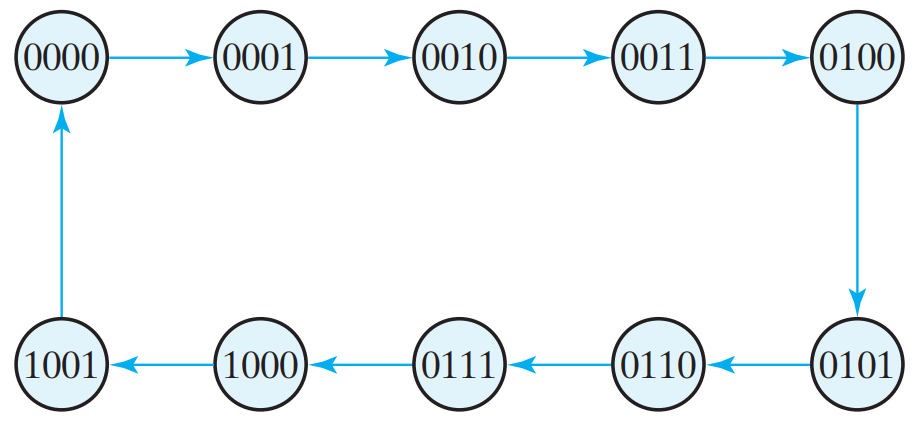
\includegraphics[width=\linewidth]{img/fig-6.9.png}
  \caption{State diagram of a decimal BCD counter}
  \label{fig:6.9}
\end{figure}

\vspace*{\fill}
\columnbreak

The logic diagram of a BCD ripple counter using JK flip-flops is shown in Fig. 10.
\begin{figure}[H]
  \centering
  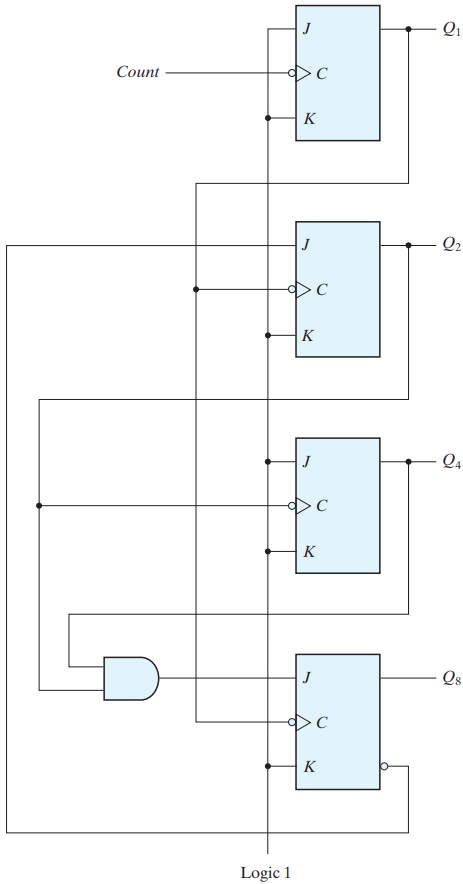
\includegraphics[width=.88\linewidth]{img/fig-6.10.png}
  \caption{BCD ripple counter}
  \label{fig:6.10}
\end{figure}

A ripple counter is an asynchronous sequential circuit. Its state changes are not synchronized to a common clock. Signals that affect the flip-flop transition depend on the way they change from 1 to 0.

The BCD counter of Fig. 10 is a \textit{decade counter}, since it counts from 0 to 9. To count in decimal from 0 to 99, we need a two-decade counter. To count from 0 to 999, we need a three-decade counter. Multiple decade counters can be constructed by connecting BCD counters in cascade, one for each decade. A three-decade counter is shown in Fig. 11. 
\begin{figure}[H]
  \centering
  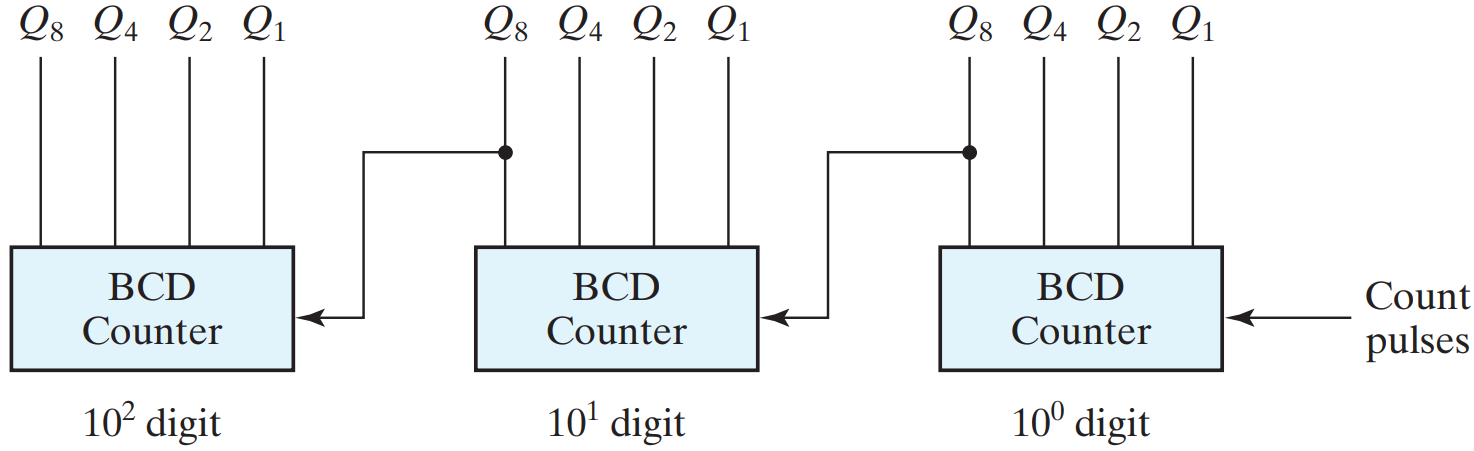
\includegraphics[width=\linewidth]{img/fig-6.11.png}
  \caption{BCD ripple counter}
  \label{fig:6.11}
\end{figure}
